
In questa appendice sono raccolte la definizione dei gruppi di omotopia e la dimostrazione della Proposizione~\ref{prop: esiste f omotopicamente non banale}. Tutte le definizioni e i risultati sono tratti da \cite{hatcher2000algebraic}, ad eccezione del Teorema~\ref{teo: approssimazione whitney} (\cite[Theorem~6.19]{lee2012smooth}).

\section{Gruppi di omotopia}

Siano \(X\) e \(Y\) due spazi topolgici e \(A \subset X\). Due mappe continue \(f,g:X \to Y\) si dicono \textit{omotope relativamente ad \(A\)} se esiste una mappa \(H:X \times [0,1] \to Y\), detta \textit{omotopia relativa ad \(A\)}, tale che
\begin{itemize}
	\item \(H(x,0) = f(x)\) per ogni \(x \in X\);
	\item \(H(x,1) = g(x)\) per ogni \(x \in X\);
	\item \(H(a,t) = f(a) = g(a)\) per ogni \(a \in A\), \(t \in [0,1]\).
\end{itemize}
È immediato verificare che questa è una relazione di equivalenza su \(C^0(X,Y)\).

Sia \(x_0 \in X\) un punto fissato. La coppia \((X,x_0)\) è detta \textit{spazio puntato}, e \(x_0\) è detto \textit{punto base}. Sia \((Y,y_0)\) un altro spazio puntato. Una mappa tra spazi puntati \(f:(X,x_0) \to (Y,y_0)\) è una mappa continua \(f : X \to Y\) tale che \(f(x_0)=y_0\).

Sia  \(e_n =(0,\dots,0,1)\) il polo nord della sfera \(\Sp^n \subset \R^{n+1}\). Denotiamo \(\pi_n(X,x_0)\) l'insieme di classi di omotopia relativa a \({x_0}\) di mappe tra spazi puntati \(f:(\Sp^n,e_n) \to (X,x_0)\). L'insieme \(\pi_n(X,x_0)\) eredita una struttura di gruppo se dotato dell'operazione \([f][g]=[f*g]\) (Figura \ref{fig: operazione gruppo di omotopia}), con
\begin{itemize}
	\item  \(f*g=c \circ f \vee g\);
	\item \(c:\Sp^n \to \Sp^n \) la mappa che collassa l'equatore \(\Sp^{n-1} \owns e_n\) in un punto;
	\item \(f \vee g : \Sp^n \to \Sp^n \to X\) definita come \(f\) su \(\Sp^n \vee e_n\) e \(g\) su \(e_n \vee \Sp^n\), avendo ruotato le due sfere in modo che \(e_n\) sia il punto di contatto.
\end{itemize} 

%OPERAZIONE DI GRUPPO
\begin{figure}[h]
	\centering
	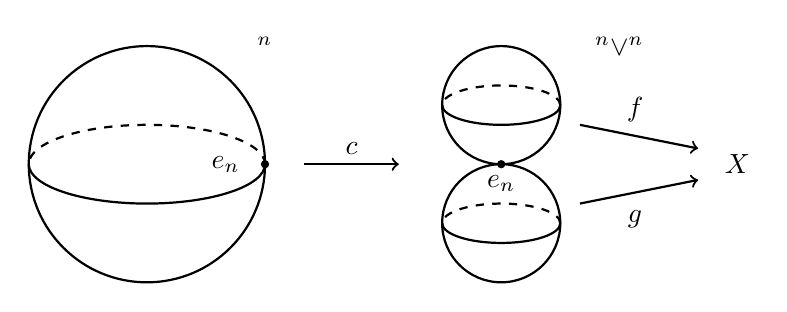
\begin{tikzpicture}
		%\draw[help lines](-2,-2) grid (10,2);
		
		%Sfera
		\draw[thick](-1.5,0)arc(180:360:1.5 and 0.5);
		\draw[thick,dashed](1.5,0)arc(0:180:1.5 and 0.5);
		\draw[thick] (0,0)circle(1.5);
		\fill (1.5,0) circle (1.5pt);
		\node at (1,0){\(e_n\)};
		\node at (1.5,1.5){\(\Sp^n\)};
		
		\draw [thick,->] (2,0)--(3.2,0);
		\node at (2.6,0.2){\(c\)};
		
		%Bouqet di sfere
		\draw[thick] (4.5,0.75)circle(0.75)
		(4.5,-0.75)circle(0.75);
		\draw[thick](3.75,0.75)arc(180:360:0.75 and 0.25)
		(3.75,-0.75)arc(180:360:0.75 and 0.25);
		\draw[thick,dashed](5.25,0.75)arc(0:180:0.75 and 0.25)
		(5.25,-0.75)arc(0:180:0.75 and 0.25);
		\fill (4.5,0) circle (1.5pt);	
		\node at (4.5,-0.25){\(e_n\)};
		\node at (6,1.5){\(\Sp^n \vee \Sp^n\)};
		
		\draw[thick,->](5.5,0.5)--(7,0.2);
		\draw[thick,->](5.5,-0.5)--(7,-0.2);
		
		\node at (6.2,0.7){\(f\)};
		\node at (6.2,-0.7){\(g\)};
		
		%X
		\node at(7.5,0){\(X\)};
	\end{tikzpicture}
	
	\caption{Operazione di gruppo su \(\pi_n(X,x_0)\).}
	\label{fig: operazione gruppo di omotopia}
\end{figure}

\begin{defi}
	\(\pi_n(X,x_0)\) è l'\(n\)-esimo \textit{gruppo di omotopia} dello spazio puntato \((X,x_0)\).
\end{defi}

\begin{oss}
	Identificando \(\Sp^1 = [0,1]/\{0,1\}\), è immediato verificare che il gruppo fondamentale è esattamente il primo gruppo di omotopia. 
\end{oss}

\begin{prop}\label{prop: invarianza pt base}
	Una cammino \(\gamma: [0,1] \to X\), con \(x_0 = \gamma(0)\) e \(x_1=\gamma(1)\), induce isomorfismi \(\pi_n \gamma: \pi_n(X,x_1) \to \pi_n(X,x_0)\), definiti come in Figura~\ref{fig: cambio punto base}.
\end{prop}
Per la dimostrazione si veda \cite[p. 341]{hatcher2000algebraic}.


	\begin{figure}[h]
	\centering
	\begin{tikzpicture}[decoration={markings, mark=at position 0.5 with {\arrow{<}}}]
		\draw[thick](-2,-2) rectangle (2,2);
		\draw[thick](-1,-1) rectangle (1,1);
		\draw[thin](-1,-1) to (-2,-2);
		\draw[thin](1,-1) to (2,-2);
		\draw[thin](-1,1) to (-2,2);
		\draw[thin](1,1) to (2,2);
		\draw[thin](-1,0) to (-2,0);
		\draw[thin](0,-1) to (0,-2);
		\draw[thin](1,0) to (2,0);
		\draw[thin](0,1) to (0,2);
		\draw[thin](-0.5,-1) to (-1,-2);
		\draw[thin](0.5,-1) to (1,-2);
		\draw[thin](1,-0.5) to (2,-1);
		\draw[thin](1,0.5) to (2,1);
		\draw[thin](0.5,1) to (1,2);
		\draw[thin](-0.5,1) to (-1,2);
		\draw[thin](-1,0.5) to (-2,1);
		\draw[thin](-1,-0.5) to (-2,-1);
		\draw[thin,decorate](-1,-1) to (-2,-2);
		\draw[thin,decorate](1,-1) to (2,-2);
		\draw[thin,decorate](-1,1) to (-2,2);
		\draw[thin,decorate](1,1) to (2,2);
		\draw[thin,decorate](-1,0) to (-2,0);
		\draw[thin,decorate](0,-1) to (0,-2);
		\draw[thin,decorate](1,0) to (2,0);
		\draw[thin,decorate](0,1) to (0,2);
		\draw[thin,decorate](-0.5,-1) to (-1,-2);
		\draw[thin,decorate](0.5,-1) to (1,-2);
		\draw[thin,decorate](1,-0.5) to (2,-1);
		\draw[thin,decorate](1,0.5) to (2,1);
		\draw[thin,decorate](0.5,1) to (1,2);
		\draw[thin,decorate](-0.5,1) to (-1,2);
		\draw[thin,decorate](-1,0.5) to (-2,1);
		\draw[thin,decorate](-1,-0.5) to (-2,-1);
		
		\node at (-0.7,-0.05){\(x_1\)};
		\node at (-2.3,-0.05){\(x_0\)};
		\node at (0.7,0.05){\(x_1\)};
		\node at (2.3,0.05){\(x_0\)};
		\node at (0,-0.7){\(x_1\)};
		\node at (0,-2.3){\(x_0\)};
		\node at (0,0.7){\(x_1\)};
		\node at (0,2.3){\(x_0\)};
		\node at (-1.5, 0.3){\(\gamma\)};
		\node at (0,0){\(f\)};
		
	\end{tikzpicture}
	
	\caption{Identificando \(\Sp^n = I^n/ \de I^n\), con \(I=[0,1]\), possiamo lavorare sull'ipercubo \(I^n\). Dunque la figura definisce, per ogni \(f : (\Sp^n,e_n) \to (X,x_1)\), una mappa continua \(\gamma f: (\Sp^n,e_n) \to (X,x_0)\) e possiamo definire \(\pi_n\gamma[f] \coloneq [\gamma f]\).}
	\label{fig: cambio punto base}
\end{figure}

Qualora \(X\) sia connesso per archi, la Proposizione~\ref{prop: invarianza pt base} permette di denotare l'\(n\)-esimo gruppo di omotopia \(\pi_n(X)\), senza specificare il punto base. In quanto segue, se \(X\) è connesso per archi, adotteremo questa notazione.

Concludiamo la sezione con il seguente risultato di approssimazione.

\begin{teo}[di approssimazione di Whitney]\label{teo: approssimazione whitney}
	Siano \(N,M\) due varietà differenziabili e sia \(F:N \to M\) una mappa continua. Allora \(F\) è omotopa a una mappa liscia \(\widetilde{F}:N \to M\). Inoltre, se \(F\) è \(C^\infty\) su un sottoinsieme chiuso \(A \subset N\), allora l'omotopia può essere scelta relativa ad \(A\), e in particolare \(\widetilde{F}|_A = F|_A\).
\end{teo}
\begin{proof}
	Si veda \cite[Theorem 6.19]{lee2012smooth}.
\end{proof}

Scegliendo \(N=\Sp^k\) e \(A=\{e_k\}\) otteniamo il seguente corollario.
\begin{cor}\label{cor: rappresentazione liscia}
	Se \(M\) è una varietà differenziabile, ogni classe \(\alpha \in \pi_k(M,p)\) ammette un rappresentante in \(C^\infty(\Sp^k,M)\). 
\end{cor}

\section{Gruppi di omotopia di una varietà semplicemente connessa}

Lo scopo di questa sezione è dimostrare la seguente:

\begin{prop}\label{prop: esiste f omotopicamente non banale}
	Se \(M\) è una varietà (topologica) \(n\)-dimensionale, chiusa e semplicemente connessa, allora esiste \(0<k < n\) tale che \(\pi_{k+1}(M) \not = \{0\}\). In particolare, se \(M\) è una varietà differenziabile, esiste una mappa \(f:\Sp^{k+1} \to M\) di classe \(C^\infty\) e omotopicamente non banale, cioè non omotopa relativamente al punto \(e_{k+1} \in \Sp^{k+1}\) a nessuna mappa costante. 
\end{prop}

Per dimostrarlo, utilizzeremo risultati profondi che connettono tra loro \textit{omotopia} e \textit{omologia}. Poiché per la comprensione dell'enunciato della Proposizione~\ref{prop: esiste f omotopicamente non banale} non è rilevante sapere cosa sono i gruppi di omologia \(H_k(X)\), li tratteremo semplicemente come dei gruppi associati a uno spazio topologico \(X\), rimandando a \cite{hatcher2000algebraic} per tutte le definizioni. 

Riportiamo i seguenti risultati, senza dimostrazione.

\begin{teo} \label{teo: H_n = Z}
	Se \(M\) è una varietà \(n\)-dimensionale chiusa e semplicemente connessa, allora \(H_n(M) \cong \Z\).
\end{teo}
Per la dimostrazione, si veda \cite[Proposition 3.25 e Theorem 3.26]{hatcher2000algebraic}.

\begin{teo}[Hurewicz]\label{teo: Hurewizc}
	Sia \(X\) uno spazio topologico connesso per archi e tale che \(\pi_k(X)=\{0\}\) per ogni \(k \leq n-1\). Allora \(\pi_n(X)\cong H_n(X)\). 
\end{teo}
Per la dimostrazione, si veda \cite[Theorem 4.32]{hatcher2000algebraic}.

\begin{proof}[Dimostrazione della Proposizione~\ref{prop: esiste f omotopicamente non banale}]
	Supponiamo che \(\pi_{k+1}(M)\) siano banali per ogni \(k < n-1\) e mostriamo che \(\pi_n(M) \not= \{0\}\). Per il teorema di Hurewicz, \(\pi_n(M) \cong H_n(M)\), che, per il Teorema~\ref{teo: H_n = Z}, è isomorfo a \(\Z\).
	
	Sia \(M\) una varietà differenziabile \(n\)-dimensionale, chiusa e semplicemente connessa. Abbiamo provato che esiste \(0<k<n\) tale che \(\pi_{k+1}(M) \neq \{0\}\). Concludiamo con il Corollario \ref{cor: rappresentazione liscia} scegliendo un rappresentante liscio di una classe non banale \(\alpha \in \pi_{k+1}(M,p)\). 
\end{proof}